\documentclass[runningheads]{llncs}

\usepackage[T1]{fontenc}
\usepackage{graphicx}
\usepackage{booktabs}
\usepackage{tabularx}
\usepackage{multirow}
\usepackage{amsmath}
\usepackage{amssymb}
\usepackage{xcolor}
\usepackage{url}
\usepackage{hyperref}

\hypersetup{
  colorlinks=true,
  linkcolor=blue,
  citecolor=blue,
  urlcolor=blue
}

\newcommand{\revisiontext}[1]{\textcolor{blue}{#1}}

\title{Unified Coarse-to-Fine Landmark Localization for Multi-Domain Ultrasound Biometry}

\titlerunning{Unified Coarse-to-Fine Ultrasound Biometry}

\author{
Hamza Rasaee\inst{1}
\and
Hassan Rivaz\inst{1}
}

\authorrunning{H. Rasaee and H. Rivaz}

\institute{
Department of Electrical and Computer Engineering, Concordia University, Montreal, Canada\\
\email{\{hamza.rasaee,hassan.rivaz\}@concordia.ca}
}

\begin{document}
\maketitle

\begin{abstract}
\noindent Ultrasound biometry requires accurate localization of anatomical landmarks across fetal, intrapartum, and cardiac imaging protocols. The target structures range from short endpoint measurements to dense multi-landmark cardiac configurations, while ultrasound appearance varies across devices, acquisition settings, and patients. We propose a unified single-checkpoint landmark localization model that combines a shared public DINOv3 vision transformer encoder, task-specific feature pyramid necks, context-local task adaptation, high-resolution heatmaps, and learned \revisiontext{coordinate} refinement. The model uses one shared representation and one trained checkpoint for all regression subsets; task identity selects internal prediction heads rather than independent expert checkpoints. On the \revisiontext{organizer-confirmed released annotation evaluation} covering nine task subsets, the selected DINOv3 Vision Transformer Base (ViT-B) model achieves an average Mean Radial Error (MRE) of \revisiontext{5.70} pixels. The same single checkpoint achieved 24.77 on public validation and 23.29 on the final-test Docker evaluation. These results show that publicly pretrained transformer features, high-resolution \revisiontext{coordinate} refinement, and controlled task-specific decoding provide an effective unified model for general ultrasound biometry.

\keywords{Ultrasound Biometry \and Multi-Task Learning \and DINOv3 \and Landmark Localization \and Vision Transformers}
\end{abstract}

\section{Introduction}
Ultrasound biometry converts anatomical appearance into reproducible geometric measurements, such as endpoints, diameters, angles, and multi-landmark contours. These measurements are central to fetal, intrapartum, and cardiac assessment, but their automation remains difficult because ultrasound images contain speckle, shadowing, missing boundaries, device-dependent contrast, and strong protocol variation. This makes multi-domain ultrasound biometry a useful test case for whether a single model can combine general visual representation learning with precise, task-specific geometric prediction.

The Foundation Model for Ultrasound Biometry benchmark exposes this difficulty. A single submission must process the challenge task families represented by nine landmark-regression subsets whose labels range from two endpoints to dense cardiac configurations. The official objective combines landmark MRE with derived measurement Mean Absolute Error (MAE), so a useful model must localize points accurately and preserve clinical measurement geometry. Separate anatomy-specific networks do not satisfy the intended single-model setting, whereas a fully shared decoder may ignore task-specific geometry.

We address this trade-off with a unified coarse-to-fine landmark model. The system combines a shared public DINOv3 encoder with task-specific spatial aggregation and high-resolution heatmap-plus-offset decoding for sub-pixel landmarks. The task-specific components are internal modules inside one trained network and one checkpoint. The method does not route images to independent dataset-specific checkpoints, does not ensemble separately trained models, and does not manually correct predictions. The main contribution is therefore a complete single-checkpoint design for heterogeneous ultrasound landmark biometry with controlled task specialization.

\section{Related Work}
Ultrasound biometry has traditionally been organized around anatomy- and protocol-specific measurements. Recent clinical guidelines define standardized fetal and cardiac ultrasound views and specify how geometric quantities should be obtained from these images~\cite{isuog2023cardiac}. Deep learning has also been used for ultrasound view recognition and localization, as in SonoNet for fetal standard plane analysis~\cite{baumgartner2017sononet}. These works demonstrate the value of task-specific ultrasound modeling, but the setting considered here is broader: the model must handle multiple anatomical domains and landmark geometries within one unified model.

Landmark localization provides a natural representation for this problem because points can be evaluated directly and converted into downstream biometric measurements. Heatmap regression has been a dominant approach for accurate landmark and keypoint prediction because it preserves spatial uncertainty and provides dense supervision~\cite{payer2016regressing,newell2016hourglass,sun2019hrnet}. Center-based and object-as-points formulations further show that compact dense prediction can recover precise coordinates from image features~\cite{zhou2019objects}. Structured landmark methods are especially relevant for ultrasound because they incorporate spatial configuration when local appearance is ambiguous~\cite{payer2019integrating}. Recent DINO-based medical tracking work also shows that self-supervised transformer features can provide robust explicit correspondences for anatomical motion estimation in cine medical imaging~\cite{salari2025dinomotion}. Our method follows this heatmap-based line, but extends it with high-resolution outputs and learned offsets so that the final coordinates are less limited by heatmap discretization.

The encoder design is motivated by progress in self-supervised vision transformers. ViT, DINO, DINOv2, and DINOv3 show that transformer representations can transfer across visual domains and support dense downstream prediction~\cite{dosovitskiy2021vit,caron2021dino,oquab2024dinov2,simeoni2025dinov3}. Recent ultrasound studies from our group also showed the value of multi-task supervision, semi-supervised representation learning, and prompt-driven foundation models for ultrasound analysis~\cite{behboodi2021breast,rasaee2025sarcopenia,rasaee2025grounding}. For our landmark task, the model must transform transferable image features into a small set of measurement-defining points. We therefore use a public DINOv3 vision transformer as the shared encoder and attach task-specific spatial prediction modules within the same checkpoint.

The multi-task aspect is equally important. Classical hard parameter sharing can improve data efficiency but can also underfit tasks with different label structure, whereas cross-stitch connections and uncertainty-based weighting provide mechanisms for balancing related objectives~\cite{caruana1997,misra2016crossstitch,kendall2018multitask}. The Foundation Model for Ultrasound Biometry setting has exactly this tension: all tasks share ultrasound statistics, but their landmark counts, spatial layouts, and measurement semantics differ substantially. Our architecture therefore keeps one shared pretrained encoder while allowing task-specific feature aggregation and task-conditioned decoding where geometry requires it.

\section{Method}
\subsection{Problem formulation}
\label{sec:problem-formulation}
Each training image belongs to one of nine landmark-regression subsets: apical four-chamber view (A4C), angle of progression (AOP), fetal abdomen (FA), the released two-point cervical-length subset (FUGC), head circumference (HC), inferior vena cava (IVC), parasternal long-axis view (PLAX), parasternal short-axis view (PSAX), or fetal femur length (\texttt{fetal\_femur}). For an image $I_i$ with task label $t_i$, the annotation is a set of $K_{t_i}$ two-dimensional landmarks $\mathbf{Y}_i \in \mathbb{R}^{K_{t_i}\times 2}$, where $K_t$ ranges from two to twenty-two. We cast all subsets into a common heatmap-based landmark regression framework. The task identity determines the number of active landmarks, the feature neck, and the decoder, while the encoder, training objective, and exported checkpoint remain unified. All landmark coordinates are transformed into the letterboxed input coordinate system during training and are transformed back to the original image system for evaluation export.

\subsection{Model overview}
The final architecture is a single multi-task network with a shared DINOv3 ViT-B encoder. Given an image and task identifier, a task-specific FPN converts transformer features into a dense map, a context-local adapter injects local image evidence, and the selected decoder predicts landmark heatmaps. The selected configuration uses 512\,$\times$\,512 letterboxed inputs and 128\,$\times$\,128 heatmaps. A learned offset branch refines the soft-argmax coordinate to reduce heatmap discretization error. Figure~\ref{fig:overview} summarizes the unified setup.

\begin{figure}[t]
  \centering
  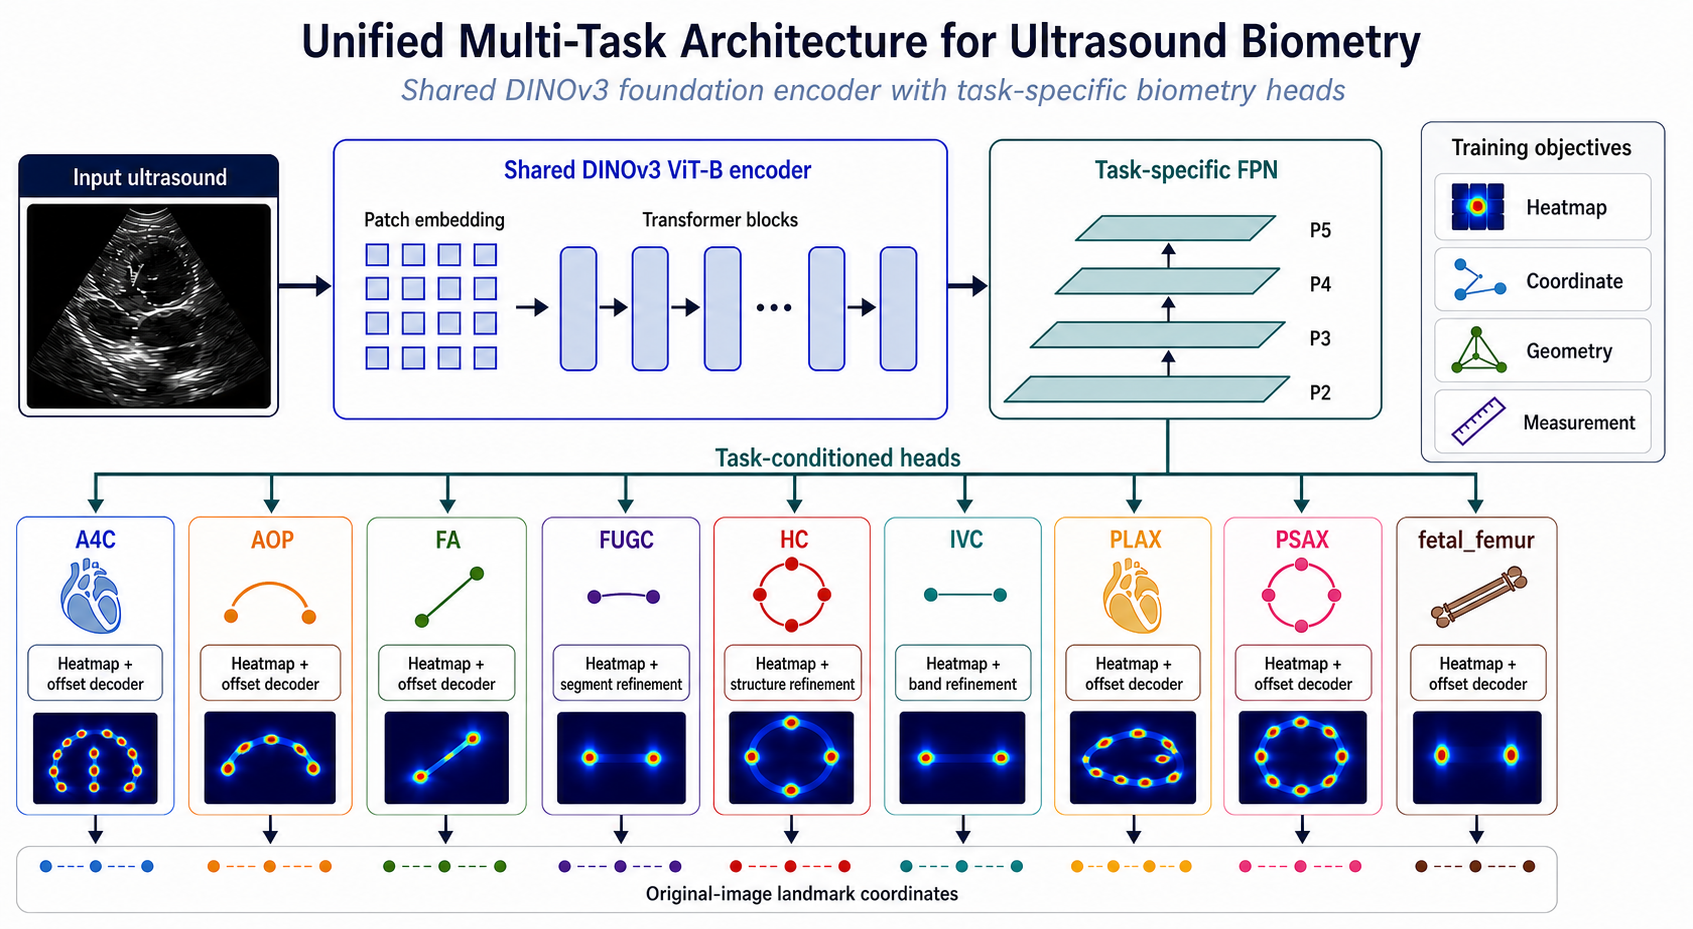
\includegraphics[width=\textwidth]{assets/fu_biometry_dedicated_heads_academic_imagegen_v2.png}
  \caption{Overview of the compliant single-checkpoint architecture. An ultrasound image is processed by a shared public DINOv3 ViT-B encoder and task-specific feature pyramid necks. The pyramid levels P2--P5 denote progressively coarser multi-scale feature maps, with P2 preserving the highest spatial resolution and P5 carrying the most compressed semantic representation. Task identity activates lightweight internal heads for A4C, AOP, FA, FUGC, HC, IVC, PLAX, PSAX, and fetal femur landmark prediction. \revisiontext{Generic heads and A4C use learned offsets, whereas FUGC, HC, and IVC use segment-, structure-, and band-oriented coordinate refinement, respectively.} These heads are part of one unified trained model rather than separate routed checkpoints.}
  \label{fig:overview}
\end{figure}

\subsection{Shared backbone and feature neck}
The selected architecture uses DINOv3 ViT-B initialized from public pretrained weights. Task-specific FPNs recover spatial detail while the encoder remains shared, allowing each subset to balance semantic context and boundary evidence. A context-local adapter then applies a residual task-conditioned correction from the FPN feature map and input image, preserving controlled specialization inside one network. \revisiontext{The model has 144.4 million trainable parameters: the shared encoder contains 85.6 million (59.3\%), while all task-specific FPNs, adapters, and heads together contain 58.7 million (40.7\%).}

\subsection{Task-specific decoding}
The decoder profile is selected by task identity within the same checkpoint. \texttt{A4C} uses a cardiac-graph decoder, \texttt{HC} a compact-structure refinement decoder, \texttt{IVC} a band-oriented endpoint decoder, and \texttt{FUGC} a short-segment refinement decoder. The remaining subsets use high-resolution offset heatmap decoders. All decoders share the same interface: they predict landmark heatmaps and, when available, refined coordinates or auxiliary structure maps, so training and export remain unified across tasks.

\subsection{Coordinate decoding and export}
For a predicted heatmap logit map $H_k$ of landmark $k$, we convert logits to a spatial probability distribution and compute a differentiable soft-argmax coordinate:
\begin{equation}
\hat{\mathbf{c}}_k =
\sum_{\mathbf{u}\in\Omega} \mathbf{u}\,
\mathrm{softmax}(H_k)(\mathbf{u}),
\end{equation}
where $\Omega$ is the normalized 128\,$\times$\,128 heatmap grid. If a decoder predicts an offset $\Delta_k$, the final transformed coordinate is
\begin{equation}
\hat{\mathbf{p}}_k =
\mathrm{clip}(\hat{\mathbf{c}}_k+\Delta_k,0,1).
\end{equation}
This keeps coordinate extraction differentiable while allowing correction below the heatmap cell scale. \revisiontext{For generic offset heads, FPN features sampled at each soft-argmax coordinate are combined with coordinate, global-image, and landmark-index embeddings. Two graph-refinement blocks predict a bounded two-dimensional correction through a \texttt{tanh} output, with maximum normalized displacement 0.03; direct coordinate loss supervises the refined output.} During inference, the inverse letterbox transform maps predictions to original-image coordinates.

\subsection{Training objectives}
The final model is trained with a base landmark loss that combines dense heatmap supervision and direct coordinate supervision:
\begin{equation}
\mathcal{L}_{\text{base}} =
\mathcal{L}_{\text{heatmap}} + 0.2 \mathcal{L}_{\text{coord}}.
\end{equation}
\noindent
Here, $\mathcal{L}_{\text{heatmap}}$ supervises dense landmark evidence and $\mathcal{L}_{\text{coord}}$ supervises decoded coordinates. The complete objective also includes small task-aware terms:
\begin{equation}
\mathcal{L} =
\mathcal{L}_{\text{base}}
+ \lambda_m \mathcal{L}_{\text{meas}}
+ \lambda_g \mathcal{L}_{\text{geom}}.
\end{equation}
The measurement and geometry terms are used only where landmarks define distances, compact structures, short segments, vessel bands, or bone shafts. For AOP, we compute the angle between the two predicted line segments during validation and report its mean absolute error in degrees. Auxiliary terms are conservatively weighted.
\subsection{Data pipeline}
The released datasets were standardized into a unified CSV schema. Images are resized with aspect-ratio-preserving letterboxing, and landmarks use the same transform before inverse mapping to the original image. We preserve the organizer-defined landmark order, including the odd-even vertical ordering standard for cardiac landmarks \revisiontext{for final reporting}. \revisiontext{The selected checkpoint was trained on all 6768 released rows available during development, including 25 fetal-femur images later listed by the organizers as orientation anomalies;} inference remains automatic and does not manually edit predictions.

\subsection{Single-model compliance}
\label{sec:single-model-compliance}
The final Docker submission uses one trained checkpoint. Public DINOv3 ViT-B weights initialize the shared encoder; no SAM3 or other additional pretrained segmentation/text model is used. All FPNs, adapters, and heads are parameters of this checkpoint and share the encoder representation. The task identifier selects an internal head, not an independently trained task- or dataset-specific checkpoint. Training uses \revisiontext{all official challenge annotations available during model development}. We use no independent experts, checkpoint ensembles, model averaging, manual correction, static public-test predictions, or hidden-test feedback.

\section{Experiments and Results}
\subsection{Dataset and evaluation protocol}
All experiments use the public Foundation Model for Ultrasound Biometry release and the nine task subsets defined in Section~\ref{sec:problem-formulation}~\cite{fubiometrychallenge}. \revisiontext{Organizer documentation traces relevant data to JNU-IFM~\cite{lu2022jnu} and PSFHS~\cite{chen2024psfhs,bai2025psfhs}; IUGC challenge releases~\cite{bai2024iugc,bai2025iugc} and benchmark analyses~\cite{bai2026iugc,bai2026iugcBeyond}; and FUGC cervical data~\cite{bai2024fugcDataset,bai2026fugc}.} We use train/validation splits from the released annotations for model development and evaluate the selected model on the \revisiontext{organizer-confirmed} 6768-image released annotation set. The official objective combines landmark MRE and clinically derived parameter MAE with normalized aggregation; accordingly, checkpoint selection uses grouped validation splits with task-aware weighting.

\subsection{Implementation details}
Images are letterboxed to 512\,$\times$\,512, and the selected model predicts 128\,$\times$\,128 heatmaps with learned offsets. We use PyTorch~\cite{paszke2019pytorch}, AdamW with learning rate $2\times10^{-5}$, weight decay 0.01, cosine decay to $10^{-6}$, batch size four, mixed precision, gradient accumulation of one, and EMA decay 0.999. \revisiontext{The selected model was warm-started from an earlier unified 64-resolution checkpoint trained only on official annotations; compatible parameters were transferred before all 144.4 million parameters were jointly optimized.} Training uses light brightness/contrast and Gaussian-noise augmentation without geometric transforms, with early stopping \revisiontext{(patience 10 and minimum improvement 0.01)} after 12 epochs from a 2000-epoch budget. Experiments were run on NVIDIA RTX 4090 GPUs with 24 GB of memory.

\subsection{Main results}
We report released-annotation, public-validation, and final-test scores where available. Table~\ref{tab:main-results} includes only one-checkpoint variants; the final-test score is from the frozen Docker submission and was not used for model selection.

\begin{table}[t]
  \centering
  \caption{Comparison of representative single-checkpoint model variants. ``Rel.'' denotes released annotated data, ``Val.'' denotes the held-out checkpoint-selection split, ``Public'' denotes the challenge public validation score, and ``Final'' denotes the final-test Docker evaluation score.}
  \label{tab:main-results}
  \small
  \setlength{\tabcolsep}{3pt}
  \begin{tabular}{lcccc}
    \toprule
    Variant & Rel. MRE$\downarrow$ & Val. MRE$\downarrow$ & Public$\downarrow$ & Final$\downarrow$ \\
    \midrule
    Early ViT-L task-FPN baseline & \revisiontext{11.02} & 25.80 & 29.88 & -- \\
    High-resolution DINOv3 offset model & \revisiontext{5.70} & 15.62 & \textbf{24.77} & \textbf{23.29} \\
    256-resolution heatmap variant & \revisiontext{5.59} & 15.96 & 24.87 & -- \\
    \bottomrule
  \end{tabular}
\end{table}

The selected model achieved \revisiontext{5.70} average released annotation MRE, with task-level errors of \revisiontext{7.83} for \texttt{A4C}, 5.57 for \texttt{AOP}, 4.36 for \texttt{FA}, 1.71 for \texttt{FUGC}, 6.39 for \texttt{HC}, 11.44 for \texttt{IVC}, 4.12 for \texttt{PLAX}, 5.44 for \texttt{PSAX}, and 4.45 for \texttt{fetal\_femur}. \revisiontext{On the held-out checkpoint-selection split, task-averaged MRE and measurement MAE were 15.62 and 10.90 pixels, respectively.} The same evaluation gives an AOP angle MAE of 3.51 degrees. The frozen Docker submission achieved a 23.29 final-test score. Although a 256-resolution variant reduced released annotation MRE to \revisiontext{5.59} pixels, the 128-resolution model gave the better public operating point.

\subsection{Ablation findings}
The ablation study showed that task-specific FPNs, high-resolution heatmaps, learned offset refinement, and task-aware decoder specialization were the main model-side contributors. The 256-resolution variant gives the strongest released annotation MRE, while the 128-resolution offset model is used as the public-validation operating point because it generalized better on the public validation score. These findings support controlled specialization inside one shared model rather than a collection of independent task experts. \revisiontext{Because no matched one-factor run is available for every component, we do not assign isolated numerical gains to simultaneously introduced changes.}

\section{Discussion}
The results support a single-checkpoint strategy for multi-domain ultrasound biometry. The shared DINOv3 encoder supplies transferable ultrasound representations, while task-specific FPNs and decoders provide the geometry needed for heterogeneous landmark layouts. This design respects the single-model constraint because all subsets use the same checkpoint and shared encoder representation, with task identity activating only internal task-specific modules.

\revisiontext{Released MRE and challenge scores are not directly comparable: 5.70 is an unnormalized landmark distance on released annotations, whereas public and final scores aggregate normalized MRE and parameter MAE on hidden images. Hidden labels prevent a per-task decomposition; plausible contributors include acquisition-domain, image-quality, protocol, and annotation shifts. The improvement from 24.77 public validation to 23.29 final Docker evaluation provides direct evidence of frozen-checkpoint generalization.}

\revisiontext{IVC remains the highest-error released subset and has only 38 samples, while A4C and HC require consistent multi-point geometry. These cases identify limited-sample vessel localization and dense or measurement-sensitive structures as the main remaining failure modes.}

\section{Limitations and Future Work}
The final-test Docker evaluation provides the challenge estimate of hidden-set generalization, while external cohorts are still needed to assess robustness beyond the challenge distribution. Future work will explore learned task conditioning, \revisiontext{annotation-protocol and sonographer variability,} and broader validation while preserving the single-checkpoint requirement.

\section{Conclusion}
We presented a unified coarse-to-fine ultrasound biometry framework based on public DINOv3 features, task-specific feature pyramids, context-local adaptation, high-resolution heatmaps, and offset refinement. The selected DINOv3 ViT-B model achieved \revisiontext{5.70} average MRE on the \revisiontext{organizer-confirmed released annotation evaluation}, reached a 24.77 public validation score, and obtained a 23.29 final-test Docker evaluation score as a single trained checkpoint. The results support combining pretrained representations with task-specific localization modules inside one unified model for robust ultrasound biometry.

\subsection*{\revisiontext{Acknowledgements.}}
\revisiontext{Funded by B2-2004995 (Fonds de recherche du Qu\'ebec – Nature et technologies B2X-363874) and Natural Sciences and Engineering Research Council of Canada (NSERC) Discovery Grant. OpenAI's ChatGPT was used to assist with English language editing in the Introduction, Methods, and Discussion sections. The authors reviewed, verified, and revised all generated text and are responsible for the manuscript content.}

\clearpage
\bibliographystyle{splncs04}
\bibliography{references}

\end{document}
